\section{Cable Tension Constraints and Negative Tension Analysis}

\textbf{Fundamental Physical Constraint:}
A critical aspect of cable-driven systems is that cables can only pull, never push. This imposes strict inequality constraints on cable tensions:
\begin{align}
T_1 &\geq 0 \\
T_2 &\geq 0
\end{align}

\begin{figure}[htbp]
\centering
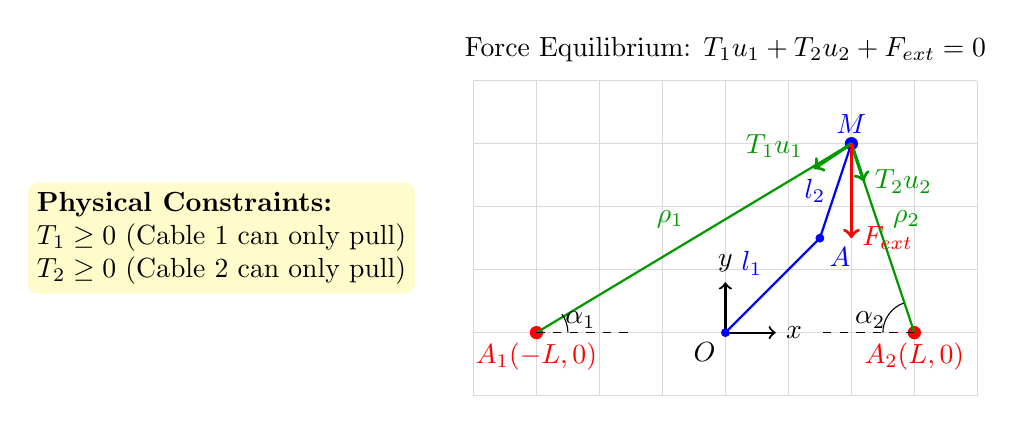
\begin{tikzpicture}[scale=0.8]
    % Grid for reference
    \draw[very thin,color=gray!30] (-4,-1) grid (4,4);
    
    % Cable anchor points
    \fill[red] (-3,0) circle (3pt) node[below] {$A_1(-L,0)$};
    \fill[red] (3,0) circle (3pt) node[below] {$A_2(L,0)$};
    
    % Base frame and robot arm (example configuration)
    \draw[thick, ->] (0,0) -- (0.8,0) node[right] {$x$};
    \draw[thick, ->] (0,0) -- (0,0.8) node[above] {$y$};
    \node[below left] at (0,0) {$O$};
    
    % Robot links (example position)
    \draw[thick, blue] (0,0) -- (1.5,1.5) node[midway, above left] {$l_1$};
    \draw[thick, blue] (1.5,1.5) -- (2,3) node[midway,  left] {$l_2$};
    
    % Joint points
    \fill[blue] (0,0) circle (2pt);
    \fill[blue] (1.5,1.5) circle (2pt) node[below right] {$A$};
    \fill[blue] (2,3) circle (3pt) node[above] {$M$};
    
    % Cables
    \draw[thick, green!60!black] (-3,0) -- (2,3) node[midway, above left] {$\rho_1$};
    \draw[thick, green!60!black] (3,0) -- (2,3) node[midway, above right] {$\rho_2$};
    
    % Cable angles
    \draw[dashed] (-3,0) -- (-1.5,0);
    \draw[dashed] (3,0) -- (1.5,0);
    \draw (-2.5,0) arc (0:36:0.5);
    \draw (2.5,0) arc (180:110:0.5);
    \node at (-2.3,0.2) {$\alpha_1$};
    \node at (2.3,0.2) {$\alpha_2$};
    
    % Cable tensions (arrows)
    \draw[->, very thick, green!60!black] (2,3) -- (1.4,2.6) node[above left] {$T_1\bm{u}_1$};
    \draw[->, very thick, green!60!black] (2,3) -- (2.2,2.4) node[right] {$T_2\bm{u}_2$};
    
    % External force
    \draw[->, very thick, red] (2,3) -- (2,1.5) node[right] {$\bm{F}_{ext}$};
    
    % Equilibrium equation
    \node[align=center] at (0,4.5) {Force Equilibrium: $T_1\bm{u}_1 + T_2\bm{u}_2 + \bm{F}_{ext} = \bm{0}$};
    
    % Constraint annotations
    \node[align=left, fill=yellow!20, rounded corners] at (-8,1.5) {
        \textbf{Physical Constraints:} \\
        $T_1 \geq 0$ (Cable 1 can only pull) \\
        $T_2 \geq 0$ (Cable 2 can only pull)
    };
\end{tikzpicture}
\caption{Cable tension force equilibrium at end-effector point M. The system must satisfy both force equilibrium and non-negative tension constraints simultaneously.}
\label{fig:cable_tension_equilibrium}
\end{figure}

\subsection{Negative Cable Tension Problem}
When mathematical analysis yields negative cable tensions, the system cannot achieve the desired force equilibrium through cables alone. This represents a fundamental limitation of cable actuation.

\textbf{Force Equilibrium Equations:}
For static equilibrium at the end-effector point M under external load $\bm{F}_{ext}$:
\begin{align}
\bm{F}_1 + \bm{F}_2 + \bm{F}_{ext} &= \bm{0} \\
T_1 \bm{u}_1 + T_2 \bm{u}_2 + \bm{F}_{ext} &= \bm{0}
\end{align}

Expanding in component form:
\begin{align}
T_1 \frac{x_M + L}{\rho_1} + T_2 \frac{x_M - L}{\rho_2} &= -F_{ext,x} \\
T_1 \frac{y_M}{\rho_1} + T_2 \frac{y_M}{\rho_2} &= -F_{ext,y}
\end{align}

\subsection{Solving for Cable Tensions}

The goal is to determine the cable tensions $T_1$ and $T_2$ required to maintain equilibrium at the end-effector point $M$ under an external force $\bm{F}_{ext} = [F_{ext,x}, F_{ext,y}]^T$. This is solved using static equilibrium conditions.

\subsubsection{Force Equilibrium at End-Effector}

At point $M$, the sum of all forces must equal zero:
\begin{align}
T_1 \bm{u}_1 + T_2 \bm{u}_2 + \bm{F}_{ext} = \bm{0}
\end{align}

Where $\bm{u}_1$ and $\bm{u}_2$ are unit vectors along the cable directions:
\begin{align}
\bm{u}_1 &= \frac{1}{\rho_1} \begin{bmatrix} x_M + L \\ y_M \end{bmatrix} \\
\bm{u}_2 &= \frac{1}{\rho_2} \begin{bmatrix} x_M - L \\ y_M \end{bmatrix}
\end{align}

\subsubsection{Matrix Formulation (Recommended for Implementation)}

The force equilibrium can be expressed as a 2×2 linear system:
\begin{align}
\begin{bmatrix}
\frac{x_M + L}{\rho_1} & \frac{x_M - L}{\rho_2} \\
\frac{y_M}{\rho_1} & \frac{y_M}{\rho_2}
\end{bmatrix} \begin{bmatrix} T_1 \\ T_2 \end{bmatrix} = -\begin{bmatrix} F_{ext,x} \\ F_{ext,y} \end{bmatrix}
\end{align}

This can be written compactly as:
\begin{align}
\bm{G}_{\rho}(\bm{q}, \bm{\rho}) \begin{bmatrix} T_1 \\ T_2 \end{bmatrix} = -\bm{F}_{ext}
\end{align}

Where $\bm{G}_{\rho}$ is the **Cable Geometry Jacobian** (also called the Constraint Jacobian), which maps cable tensions to end-effector forces.

\subsubsection{Direct Solution via Matrix Inversion}

Solving for tensions by inverting the Cable Geometry Jacobian:
\begin{align}
\begin{bmatrix} T_1 \\ T_2 \end{bmatrix} &= -\bm{G}_{\rho}^{-1}(\bm{q}, \bm{\rho}) \begin{bmatrix} F_{ext,x} \\ F_{ext,y} \end{bmatrix}
\end{align}

The determinant and inverse of the Cable Geometry Jacobian:
\begin{align}
\det(\bm{G}_{\rho}) &= \frac{1}{\rho_1 \rho_2} \left[ \frac{x_M + L}{\rho_1} \cdot \frac{y_M}{\rho_2} - \frac{x_M - L}{\rho_2} \cdot \frac{y_M}{\rho_1} \right] \\
&= \frac{y_M}{\rho_1^2 \rho_2^2} \left[ (x_M + L) - (x_M - L) \right] \\
&= \frac{2L y_M}{\rho_1^2 \rho_2^2}
\end{align}

The matrix inverse:
\begin{align}
\bm{G}_{\rho}^{-1} &= \frac{\rho_1 \rho_2}{2L y_M} \begin{bmatrix}
\frac{y_M}{\rho_2} & -\frac{x_M - L}{\rho_2} \\
-\frac{y_M}{\rho_1} & \frac{x_M + L}{\rho_1}
\end{bmatrix}
\end{align}

\subsubsection{Explicit Cable Tension Formulas}

Multiplying out the matrix inversion:
\begin{align}
T_1 &= -\frac{\rho_1}{2L} \left[ F_{ext,x} \frac{y_M}{\rho_2} - F_{ext,y} \frac{x_M - L}{\rho_2} \right] \\
&= \frac{\rho_1}{2L y_M} \left[ F_{ext,x} y_M - F_{ext,y} (x_M - L) \right] \\
T_2 &= -\frac{\rho_2}{2L} \left[ -F_{ext,x} \frac{y_M}{\rho_1} + F_{ext,y} \frac{x_M + L}{\rho_1} \right] \\
&= \frac{\rho_2}{2L y_M} \left[ F_{ext,x} y_M + F_{ext,y} (x_M + L) \right]
\end{align}

\subsubsection{Numerical Example}

\textbf{Given Configuration:}
\begin{itemize}
    \item Link lengths: $l_1 = 1$ m, $l_2 = 1$ m
    \item Cable anchor separation: $2L = 4$ m (so $L = 2$ m)
    \item Joint configuration: $q_1 = 30^{\circ}$, $q_2 = 45^{\circ}$
    \item External load: $\bm{F}_{ext} = [10, -5]^T$ N (rightward and downward)
\end{itemize}

\textbf{Step 1: Calculate end-effector position}
\begin{align}
x_M &= l_1 \cos(30^{\circ}) + l_2 \cos(75^{\circ}) = 0.866 + 0.259 = 1.125 \text{ m} \\
y_M &= l_1 \sin(30^{\circ}) + l_2 \sin(75^{\circ}) = 0.500 + 0.966 = 1.466 \text{ m}
\end{align}

\textbf{Step 2: Calculate cable lengths}
\begin{align}
\rho_1 &= \sqrt{(x_M + L)^2 + y_M^2} = \sqrt{(1.125 + 2)^2 + 1.466^2} = \sqrt{11.383} = 3.374 \text{ m} \\
\rho_2 &= \sqrt{(x_M - L)^2 + y_M^2} = \sqrt{(1.125 - 2)^2 + 1.466^2} = \sqrt{2.591} = 1.610 \text{ m}
\end{align}

\textbf{Step 3: Apply tension formulas}
\begin{align}
T_1 &= \frac{3.374}{2 \cdot 2 \cdot 1.466} \left[ 10 \cdot 1.466 - (-5) \cdot (1.125 - 2) \right] \\
&= \frac{3.374}{5.864} \left[ 14.66 + 4.4375 \right] \\
&= 0.575 \times 19.0975 = 10.98 \text{ N} \\
T_2 &= \frac{1.610}{2 \cdot 2 \cdot 1.466} \left[ 10 \cdot 1.466 + (-5) \cdot (1.125 + 2) \right] \\
&= \frac{1.610}{5.864} \left[ 14.66 - 15.625 \right] \\
&= 0.275 \times (-0.965) = -0.265 \text{ N}
\end{align}

\textbf{Result:} $T_1 = 10.98$ N (feasible), $T_2 = -0.265$ N (**negative - infeasible!**)

This configuration would require cable 2 to push, which is physically impossible. The end-effector cannot maintain equilibrium under this force with these joint angles.

\subsubsection{Stability and Computational Considerations}

\textbf{Singularity Issues:}
The Cable Geometry Jacobian becomes singular when:
\begin{align}
\det(\bm{G}_{\rho}) = \frac{2L y_M}{\rho_1^2 \rho_2^2} = 0
\end{align}

This occurs when $y_M = 0$, meaning the end-effector is on the horizontal line through the cable anchors. At this configuration, the cables cannot support vertical forces.

\textbf{Condition Number:}
To assess numerical stability, compute the condition number:
\begin{align}
\kappa(\bm{G}_{\rho}) = \|\bm{G}_{\rho}\| \cdot \|\bm{G}_{\rho}^{-1}\|
\end{align}

A high condition number indicates ill-conditioning and sensitivity to numerical errors. Avoid configurations where $\kappa > 100$.

\textbf{Computational Algorithm:}

\begin{algorithm}[H]
\caption{Cable Tension Computation and Feasibility Analysis}
\label{alg:cable_tension}
\begin{algorithmic}[1]
\REQUIRE Joint configuration $\bm{q} = [q_1, q_2]^T$, external force $\bm{F}_{ext} = [F_{ext,x}, F_{ext,y}]^T$
\REQUIRE Link lengths $l_1, l_2$, cable anchor separation $2L$, singularity tolerance $\epsilon_{sing}$
\ENSURE Cable tensions $T_1, T_2$ and feasibility status

\STATE \textbf{Step 1: Forward Kinematics}
\STATE $x_M \leftarrow l_1 \cos(q_1) + l_2 \cos(q_1 + q_2)$
\STATE $y_M \leftarrow l_1 \sin(q_1) + l_2 \sin(q_1 + q_2)$

\STATE \textbf{Step 2: Cable Length Computation}
\STATE $\rho_1 \leftarrow \sqrt{(x_M + L)^2 + y_M^2}$
\STATE $\rho_2 \leftarrow \sqrt{(x_M - L)^2 + y_M^2}$

\STATE \textbf{Step 3: Cable Geometry Jacobian Construction}
\STATE $\bm{G}_{\rho} \leftarrow \begin{bmatrix}
\frac{x_M + L}{\rho_1} & \frac{x_M - L}{\rho_2} \\
\frac{y_M}{\rho_1} & \frac{y_M}{\rho_2}
\end{bmatrix}$

\STATE \textbf{Step 4: Singularity Check}
\STATE $\det_{\rho} \leftarrow \text{determinant}(\bm{G}_{\rho}) = \frac{2L y_M}{\rho_1^2 \rho_2^2}$

\IF{$|\det_{\rho}| < \epsilon_{sing}$}
    \STATE \textbf{return} \{status: SINGULAR, $T_1$: undefined, $T_2$: undefined\}
    \STATE \textbf{// Configuration is singular - cannot solve for tensions}
\ENDIF

\STATE \textbf{Step 5: Solve Linear System via LU Decomposition}
\STATE $[\bm{L}, \bm{U}] \leftarrow \text{LU}(\bm{G}_{\rho})$
\STATE $\bm{y} \leftarrow \text{ForwardSubstitution}(\bm{L}, -\bm{F}_{ext})$
\STATE $\begin{bmatrix} T_1 \\ T_2 \end{bmatrix} \leftarrow \text{BackSubstitution}(\bm{U}, \bm{y})$

\STATE \textbf{Step 6: Feasibility Assessment}
\IF{$T_1 \geq 0$ \textbf{and} $T_2 \geq 0$}
    \STATE $\text{feasible} \leftarrow \text{TRUE}$
\ELSE
    \STATE $\text{feasible} \leftarrow \text{FALSE}$
    \STATE \textbf{// Record which tensions are negative}
    \IF{$T_1 < 0$} \STATE $\text{reason} \leftarrow \text{``Cable 1 would require push''}$ \ENDIF
    \IF{$T_2 < 0$} \STATE $\text{reason} \leftarrow \text{``Cable 2 would require push''}$ \ENDIF
\ENDIF

\STATE \textbf{Step 7: Condition Number Assessment (Optional)}
\STATE $\kappa \leftarrow \text{conditionNumber}(\bm{G}_{\rho})$
\IF{$\kappa > 100$}
    \STATE $\text{stability} \leftarrow \text{``ILL-CONDITIONED''}$
\ELSE
    \STATE $\text{stability} \leftarrow \text{``WELL-CONDITIONED''}$
\ENDIF

\STATE \textbf{return} $\{T_1, T_2, \text{feasible}, \text{stability}, \kappa\}$
\end{algorithmic}
\end{algorithm}

\subsubsection{Algorithm Details and Implementation Notes}

\textbf{Forward Kinematics Computation:}
The end-effector position is computed from joint angles using standard 2-DOF planar arm kinematics:
\begin{align}
x_M &= l_1 \cos(q_1) + l_2 \cos(q_1 + q_2) \\
y_M &= l_1 \sin(q_1) + l_2 \sin(q_1 + q_2)
\end{align}

\textbf{Cable Length Calculation:}
Euclidean distance from cable anchor points to end-effector:
\begin{align}
\rho_1 &= \|(x_M, y_M) - (-L, 0)\| = \sqrt{(x_M + L)^2 + y_M^2} \\
\rho_2 &= \|(x_M, y_M) - (L, 0)\| = \sqrt{(x_M - L)^2 + y_M^2}
\end{align}

\textbf{Singularity Detection:}
When $|\det(\bm{G}_{\rho})| < \epsilon_{sing}$ (typically $\epsilon_{sing} = 10^{-6}$):
\begin{align}
\frac{2L y_M}{\rho_1^2 \rho_2^2} \approx 0 \quad \Rightarrow \quad y_M \approx 0
\end{align}
This indicates the end-effector is near the line connecting cable anchors, where cable geometry cannot support arbitrary forces.

\textbf{Numerical Solution:}
LU decomposition is preferred over direct matrix inversion for numerical stability:
\begin{itemize}
    \item \textbf{Computational Cost}: $\mathcal{O}(n^3)$ for LU factorization (here $n=2$ is small)
    \item \textbf{Numerical Stability}: Better conditioning than explicit inversion
    \item \textbf{Reusability}: If multiple forces are applied with same configuration, LU factors can be reused
\end{itemize}

\textbf{Feasibility Criteria:}
\begin{align}
\text{Configuration is feasible} \iff T_1 \geq 0 \text{ and } T_2 \geq 0
\end{align}

\textbf{Condition Number Interpretation:}
\begin{align}
\kappa(\bm{G}_{\rho}) = \begin{cases}
< 10 & \text{Excellent conditioning} \\
10 - 100 & \text{Good conditioning} \\
100 - 1000 & \text{Moderate conditioning - use caution} \\
> 1000 & \text{Poor conditioning - near singularity}
\end{cases}
\end{align}

\subsubsection{Python Implementation Pseudocode}

\begin{verbatim}
def compute_cable_tensions(q1, q2, F_ext_x, F_ext_y, l1, l2, L, eps_sing=1e-6):
    """
    Compute cable tensions and feasibility for given configuration and external force.
    
    Parameters:
        q1, q2: Joint angles [rad]
        F_ext_x, F_ext_y: External force components [N]
        l1, l2: Link lengths [m]
        L: Half-distance between cable anchors [m]
        eps_sing: Singularity tolerance
    
    Returns:
        T1, T2: Cable tensions [N]
        feasible: Boolean indicating if tensions are non-negative
        det_G: Determinant of Cable Geometry Jacobian
        kappa: Condition number
    """
    # Step 1: Forward kinematics
    x_M = l1 * cos(q1) + l2 * cos(q1 + q2)
    y_M = l1 * sin(q1) + l2 * sin(q1 + q2)
    
    # Step 2: Cable lengths
    rho1 = sqrt((x_M + L)**2 + y_M**2)
    rho2 = sqrt((x_M - L)**2 + y_M**2)
    
    # Step 3: Cable Geometry Jacobian
    G_rho = np.array([
        [(x_M + L)/rho1, (x_M - L)/rho2],
        [y_M/rho1, y_M/rho2]
    ])
    
    # Step 4: Singularity check
    det_G = (2 * L * y_M) / (rho1**2 * rho2**2)
    if abs(det_G) < eps_sing:
        return None, None, "SINGULAR", det_G, None
    
    # Step 5: Solve for tensions
    F_ext = np.array([[-F_ext_x], [-F_ext_y]])
    T = np.linalg.solve(G_rho, F_ext)
    T1, T2 = T[0, 0], T[1, 0]
    
    # Step 6: Check feasibility
    feasible = (T1 >= 0) and (T2 >= 0)
    
    # Step 7: Condition number
    kappa = np.linalg.cond(G_rho)
    
    return T1, T2, feasible, det_G, kappa
\end{verbatim}

\subsection{Conditions for Negative Tensions}
Cable tensions become negative when:
\begin{align}
T_1 &< 0 \quad \text{or} \quad T_2 < 0
\end{align}

This occurs when the required force direction cannot be achieved by the available cable geometry.

\begin{figure}[htbp]
\centering
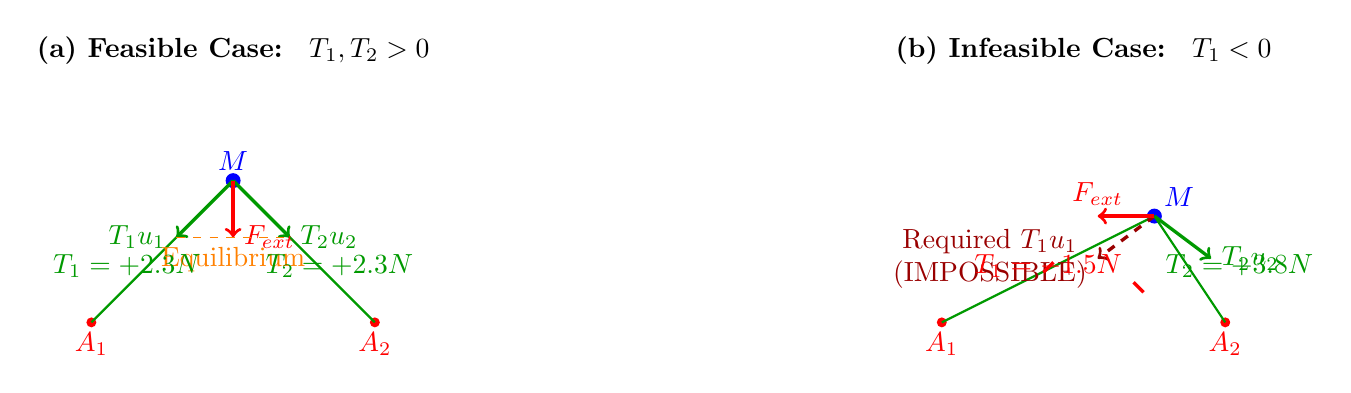
\begin{tikzpicture}[scale=0.9]
    \begin{scope}[xshift=-6cm]
        % Scenario 1: Feasible case
        \node[above] at (0,3.5) {\textbf{(a) Feasible Case: } $T_1, T_2 > 0$};
        
        % Cable anchors
        \fill[red] (-2,0) circle (2pt) node[below] {$A_1$};
        \fill[red] (2,0) circle (2pt) node[below] {$A_2$};
        
        % End-effector
        \fill[blue] (0,2) circle (3pt) node[above] {$M$};
        
        % Cables
        \draw[thick, green!60!black] (-2,0) -- (0,2);
        \draw[thick, green!60!black] (2,0) -- (0,2);
        
        % Cable forces (both pulling toward anchors)
        \draw[->, very thick, green!60!black] (0,2) -- (-0.8,1.2) node[left] {$T_1\bm{u}_1$};
        \draw[->, very thick, green!60!black] (0,2) -- (0.8,1.2) node[right] {$T_2\bm{u}_2$};
        
        % External force (downward)
        \draw[->, very thick, red] (0,2) -- (0,1.2) node[right] {$\bm{F}_{ext}$};
        
        % Force resultant (equilibrium)
        \draw[dashed, orange] (-0.8,1.2) -- (0,1.2) -- (0.8,1.2);
        \node[orange, below] at (0,1.2) {Equilibrium};
        
        % Tension values
        \node[green!60!black] at (-1.5,0.8) {$T_1 = +2.3N$};
        \node[green!60!black] at (1.5,0.8) {$T_2 = +2.3N$};
    \end{scope}
    
    \begin{scope}[xshift=6cm]
        % Scenario 2: Infeasible case
        \node[above] at (0,3.5) {\textbf{(b) Infeasible Case: } $T_1 < 0$};
        
        % Cable anchors
        \fill[red] (-2,0) circle (2pt) node[below] {$A_1$};
        \fill[red] (2,0) circle (2pt) node[below] {$A_2$};
        
        % End-effector (different position)
        \fill[blue] (1,1.5) circle (3pt) node[above right] {$M$};
        
        % Cables
        \draw[thick, green!60!black] (-2,0) -- (1,1.5);
        \draw[thick, green!60!black] (2,0) -- (1,1.5);
        
        % Required forces for equilibrium (one would need to push!)
        \draw[->, very thick, red!60!black, dashed] (1,1.5) -- (0.2,0.9) 
              node[left, align=center] {Required $T_1\bm{u}_1$ \\ (IMPOSSIBLE)};
        \draw[->, very thick, green!60!black] (1,1.5) -- (1.8,0.9) node[right] {$T_2\bm{u}_2$};
        
        % External force (leftward)
        \draw[->, very thick, red] (1,1.5) -- (0.2,1.5) node[above] {$\bm{F}_{ext}$};
        
        % Tension values
        \node[red] at (-0.5,0.8) {$T_1 = -1.5N$};
        \node[green!60!black] at (2.2,0.8) {$T_2 = +3.8N$};
        
        % Impossibility indication
        \draw[red, very thick, rotate=45] (0.1,0.9) -- (0.3,0.9);
        \draw[red, very thick, rotate=-45] (0.1,0.9) -- (0.3,0.9);
    \end{scope}
\end{tikzpicture}
\caption{Illustration of cable tension feasibility. (a) Feasible configuration where both cables can provide positive tensions. (b) Infeasible configuration where cable 1 would need to push (negative tension) to achieve equilibrium, which is physically impossible.}
\label{fig:negative_tension_cases}
\end{figure}

\textbf{Critical Geometric Conditions:}

Negative tensions typically occur when:
\begin{enumerate}
    \item \textbf{Force Direction Mismatch:} The external force requires cable compression (impossible)
    \item \textbf{Unfavorable Cable Geometry:} The cable angles $\alpha_1, \alpha_2$ create poor mechanical advantage
    \item \textbf{Serial Chain Singularities:} Robot configurations where $q_2 = 0$ or $q_2 = \pi$
    \item \textbf{Cable Anchor Proximity:} End-effector approaches the cable anchor points
    \item \textbf{Workspace Boundaries:} Near the limits of the kinematic workspace
\end{enumerate}

\subsection{Mathematical Analysis of Negative Tension Regions}

\textbf{Left Cable Tension Analysis:}
$T_1 < 0$ when:
\begin{align}
F_{ext,x} \frac{y_M}{\rho_2} - F_{ext,y} \frac{x_M - L}{\rho_2} &> 0 \\
\Rightarrow \quad F_{ext,x} y_M &> F_{ext,y} (x_M - L)
\end{align}

\textbf{Right Cable Tension Analysis:}
$T_2 < 0$ when:
\begin{align}
-F_{ext,x} \frac{y_M}{\rho_1} + F_{ext,y} \frac{x_M + L}{\rho_1} &< 0 \\
\Rightarrow \quad F_{ext,x} y_M &> F_{ext,y} (x_M + L)
\end{align}

\textbf{Critical Force Angle:}
Define the external force angle as $\beta = \text{atan2}(F_{ext,y}, F_{ext,x})$.
Negative tensions occur when the force angle is incompatible with cable directions:
\begin{align}
\text{If } \beta &\in (\alpha_1, \alpha_2) \text{ and } F_{ext} \text{ points away from cables} \\
\text{Then } T_1 &< 0 \text{ or } T_2 < 0
\end{align}

\subsection{Singularity Connection}
When cable tensions become negative, several critical situations arise:

\subsubsection{Motor Capability Loss}
The motors driving the cables cannot provide the required forces, leading to:
\begin{itemize}
    \item \textbf{Task Failure:} Inability to execute the desired motion or maintain equilibrium
    \item \textbf{Control Loss:} End-effector becomes uncontrollable in certain directions
    \item \textbf{System Instability:} Potential for unwanted oscillations or drift
    \item \textbf{Safety Issues:} Loss of load support or positioning accuracy
\end{itemize}

\subsubsection{Infinite Tension Conditions}
When the denominator in tension equations approaches zero:
\begin{align}
\sin(\alpha_2 - \alpha_1) &\to 0 \\
\Rightarrow \quad \alpha_2 &= \alpha_1 + k\pi, \quad k \in \mathbb{Z}
\end{align}

This occurs in specific geometric configurations:

\textbf{1. Parallel Cable Configuration ($\alpha_2 = \alpha_1$):}
\begin{align}
y_M &= 0 \text{ and } x_M \text{ arbitrary} \\
\text{Condition: } &\text{End-effector on X-axis between anchors}
\end{align}

\textbf{2. Anti-parallel Cable Configuration ($\alpha_2 = \alpha_1 + \pi$):}
\begin{align}
x_M &= 0 \\
\text{Condition: } &\text{End-effector on Y-axis}
\end{align}

\textbf{3. Combined Singularities:}
When cable singularities coincide with joint singularities ($q_2 = 0$ or $q_2 = \pi$), the system experiences:
\begin{itemize}
    \item Loss of multiple degrees of freedom simultaneously
    \item Reduced controllability in multiple directions
    \item Enhanced sensitivity to external disturbances
\end{itemize}

\subsection{Workspace Analysis}

\subsubsection{Workspace Definitions}
The negative tension constraint fundamentally limits the robot's operational workspace:

\textbf{Kinematic Workspace:}
\begin{align}
\mathcal{W}_{kinematic} &= \{(x_M, y_M) : |x_M^2 + y_M^2|^{1/2} \leq l_1 + l_2\} \\
&\cap \{(x_M, y_M) : |x_M^2 + y_M^2|^{1/2} \geq |l_1 - l_2|\}
\end{align}

\textbf{Feasible Workspace (for given external load):}
\begin{align}
\mathcal{W}_{feasible} &= \{(x_M, y_M) \in \mathcal{W}_{kinematic} : T_1(\bm{q}, \bm{F}_{ext}) \geq 0 \text{ and } T_2(\bm{q}, \bm{F}_{ext}) \geq 0\}
\end{align}

\textbf{Cable-Limited Regions:}
\begin{align}
\mathcal{W}_{cable-limited} &= \mathcal{W}_{kinematic} \setminus \mathcal{W}_{feasible} \\
&= \{(x_M, y_M) \in \mathcal{W}_{kinematic} : T_1(\bm{q}, \bm{F}_{ext}) < 0 \text{ or } T_2(\bm{q}, \bm{F}_{ext}) < 0\}
\end{align}

\subsubsection{Load-Dependent Workspace}
The feasible workspace depends on the external load magnitude and direction:

\textbf{Zero Load Case ($\bm{F}_{ext} = \bm{0}$):}
\begin{align}
\mathcal{W}_{feasible}(\bm{0}) = \mathcal{W}_{kinematic}
\end{align}
All kinematically reachable points are cable-feasible with zero external load.

\textbf{Gravity Load Case ($\bm{F}_{ext} = [0, -mg]^T$):}
\begin{align}
T_1 &= \frac{mg \rho_1 (x_M - L)}{2L y_M} \\
T_2 &= \frac{mg \rho_2 (x_M + L)}{2L y_M}
\end{align}

\begin{figure}[htbp]
\centering
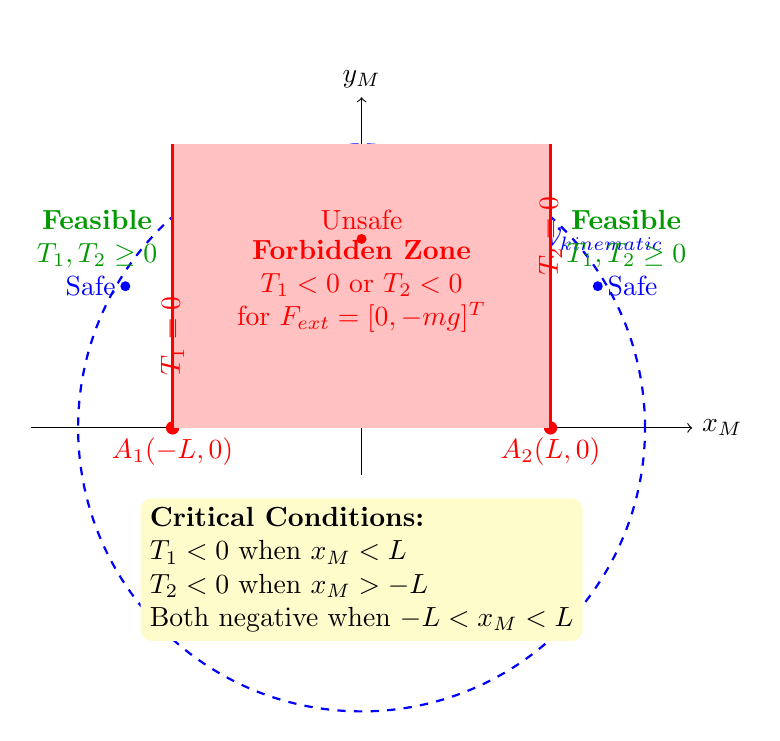
\begin{tikzpicture}[scale=1.2]
    % Coordinate system
    \draw[->] (-3.5,0) -- (3.5,0) node[right] {$x_M$};
    \draw[->] (0,-0.5) -- (0,3.5) node[above] {$y_M$};
    
    % Cable anchor points
    \fill[red] (-2,0) circle (2pt) node[below] {$A_1(-L,0)$};
    \fill[red] (2,0) circle (2pt) node[below] {$A_2(L,0)$};
    
    % Kinematic workspace (circle)
    \draw[thick, blue, dashed] (0,0) circle (3);
    \node[blue] at (2.5,2) {$\mathcal{W}_{kinematic}$};
    
    % Feasible region for downward load (outside forbidden zone)
    \fill[green!20, opacity=0.7] 
        (-2,0) -- (-2,2.236) arc (180:0:2) -- (2,0) -- (2,2.236) arc (0:180:2) -- cycle;
    \fill[white] (-2,0) rectangle (2,3);
    
    % Forbidden zone (between anchors for downward load)
    \fill[red!30, opacity=0.8] (-2,0) rectangle (2,3);
    \node[red, align=center] at (0,1.5) {\textbf{Forbidden Zone} \\ $T_1 < 0$ or $T_2 < 0$ \\ for $\bm{F}_{ext} = [0,-mg]^T$};
    
    % Boundary lines where tensions = 0
    \draw[thick, red] (-2,0) -- (-2,3) node[left, rotate=90, midway] {$T_1 = 0$};
    \draw[thick, red] (2,0) -- (2,3) node[right, rotate=90, midway] {$T_2 = 0$};
    
    % Feasible region annotation
    \node[green!60!black, align=center] at (-2.8,2) {\textbf{Feasible} \\ $T_1, T_2 \geq 0$};
    \node[green!60!black, align=center] at (2.8,2) {\textbf{Feasible} \\ $T_1, T_2 \geq 0$};
    
    % Example end-effector positions
    \fill[blue] (-2.5,1.5) circle (1.5pt) node[left] {Safe};
    \fill[red] (0,2) circle (1.5pt) node[above] {Unsafe};
    \fill[blue] (2.5,1.5) circle (1.5pt) node[right] {Safe};
    
    % Workspace boundary equations
    \node[align=left, fill=yellow!20, rounded corners] at (0,-1.5) {
        \textbf{Critical Conditions:} \\
        $T_1 < 0$ when $x_M < L$ \\
        $T_2 < 0$ when $x_M > -L$ \\
        Both negative when $-L < x_M < L$
    };
\end{tikzpicture}
\caption{Workspace analysis for downward gravitational load. The forbidden zone (red) shows regions where negative cable tensions would be required. The feasible workspace (green) is significantly reduced compared to the kinematic workspace (blue dashed circle).}
\label{fig:workspace_analysis}
\end{figure}

Negative tensions occur when:
\begin{itemize}
    \item $T_1 < 0$: when $x_M < L$ (left side of right anchor)
    \item $T_2 < 0$: when $x_M > -L$ (right side of left anchor)  
    \item Both: when $-L < x_M < L$ (between anchors)
\end{itemize}

This creates a **forbidden zone** between the cable anchors for downward loads.

\subsection{Design and Control Implications}

\subsubsection{Design Optimization}
\textbf{1. Cable Anchor Placement:}
Optimize anchor positions to maximize feasible workspace:
\begin{align}
L_{optimal} &= \arg\max_L |\mathcal{W}_{feasible}(L, \bm{F}_{ext})|
\end{align}

\textbf{2. Link Length Ratios:}
Balance serial chain workspace with cable effectiveness:
\begin{align}
\frac{l_2}{l_1} &= \arg\max_{ratio} |\mathcal{W}_{feasible} \cap \mathcal{W}_{dexterous}|
\end{align}

\textbf{3. Joint Range Limits:}
Coordinate joint limits with cable constraints:
\begin{align}
q_{2,min} &\geq \epsilon > 0 \quad \text{(avoid } q_2 = 0 \text{ singularity)} \\
q_{2,max} &\leq \pi - \epsilon \quad \text{(avoid } q_2 = \pi \text{ singularity)}
\end{align}

\subsubsection{Control Strategies}
\textbf{1. Hybrid Control Architecture:}
Switch between control modes based on tension feasibility:
\begin{algorithm}[H]
\caption{Hybrid Cable-Joint Control}
\begin{algorithmic}
\STATE \textbf{Input:} Desired end-effector position $\bm{x}_{desired}$, external load $\bm{F}_{ext}$
\STATE Compute required cable tensions $T_1, T_2$ from force equilibrium
\IF{$T_1 \geq T_{min}$ AND $T_2 \geq T_{min}$}
    \STATE Use cable control mode
    \STATE Control cable lengths $\rho_1, \rho_2$ to achieve $\bm{x}_{desired}$
\ELSE
    \STATE Use joint control mode
    \STATE Control joint angles $q_1, q_2$ to achieve $\bm{x}_{desired}$
    \STATE Set cable tensions to minimum safe values
\ENDIF
\end{algorithmic}
\end{algorithm}

\textbf{2. Pre-tensioning Strategy:}
Maintain minimum cable tensions to avoid slack and improve responsiveness:
\begin{align}
T_{1,command} &= \max(T_{1,required}, T_{min}) \\
T_{2,command} &= \max(T_{2,required}, T_{min})
\end{align}

Where $T_{min} > 0$ is the minimum safe tension level.

\textbf{3. Workspace Planning:}
Generate trajectories that avoid negative tension regions:
\begin{align}
\bm{x}_{trajectory}(t) &\in \mathcal{W}_{feasible} \quad \forall t \in [0, T_{final}]
\end{align}

\textbf{4. Redundancy Exploitation:}
Use additional degrees of freedom to maintain positive tensions:
\begin{itemize}
    \item Adjust joint configuration while maintaining end-effector position
    \item Vary cable pre-tension levels dynamically
    \item Coordinate multiple cables if available
\end{itemize}

\subsection{Practical Implementation Considerations}

\subsubsection{Sensor Requirements}
\textbf{1. Tension Monitoring:}
\begin{itemize}
    \item Load cells or strain gauges in cable paths
    \item Real-time tension feedback for control
    \item Early warning for approaching negative tension conditions
\end{itemize}

\textbf{2. Position Sensing:}
\begin{itemize}
    \item Joint angle encoders for $q_1, q_2$
    \item Cable length sensors for $\rho_1, \rho_2$
    \item End-effector position confirmation
\end{itemize}

\subsubsection{Safety Considerations}
\textbf{1. Emergency Protocols:}
\begin{itemize}
    \item Automatic joint braking when cable tensions drop
    \item Fail-safe positions with guaranteed positive tensions
    \item Load sharing between joint and cable actuators
\end{itemize}

\textbf{2. Operating Limits:}
\begin{itemize}
    \item Conservative workspace boundaries
    \item Maximum load ratings based on tension analysis
    \item Speed limitations near singular configurations
\end{itemize}

\subsubsection{Computational Requirements}
\textbf{1. Real-time Tension Calculation:}
Fast algorithms for computing required tensions:
\begin{align}
\text{Computation time: } &O(1) \text{ per control cycle} \\
\text{Memory requirement: } &O(1) \text{ for 2D system}
\end{align}

\textbf{2. Workspace Monitoring:}
Efficient methods to check feasibility:
\begin{itemize}
    \item Pre-computed workspace maps
    \item Look-up tables for common load cases
    \item Approximate analytical boundaries
\end{itemize}

\subsection{Summary}
The cable tension constraint analysis reveals that:

\textbf{Key Insights:}
\begin{enumerate}
    \item Cable systems have inherent directional limitations due to tension positivity
    \item Negative tensions create forbidden workspace regions that vary with external loads
    \item Singularities can be triggered by both geometric and force-based conditions
    \item Proper design and control can mitigate but not eliminate these constraints
\end{enumerate}

\textbf{Design Guidelines:}
\begin{enumerate}
    \item Optimize cable anchor placement for maximum feasible workspace
    \item Implement hybrid control strategies to handle tension constraints
    \item Include pre-tensioning systems for improved performance
    \item Plan trajectories considering both kinematic and force constraints
\end{enumerate}

\textbf{Future Research Directions:}
\begin{enumerate}
    \item Optimization of cable arrangements for specific task requirements
    \item Advanced control algorithms that anticipate tension constraints
    \item Integration with machine learning for adaptive workspace planning
    \item Extension to higher-DOF and 3D cable-driven systems
\end{enumerate}